\documentclass[a4paper]{article}
\usepackage[a4paper,margin=0mm]{geometry}
\usepackage{fontspec}
\usepackage{unicode-math}
\usepackage{tikz}
\usepackage[table]{xcolor}
\usepackage[absolute]{textpos}
\usepackage{array}

\setmainfont{Libertinus Serif}
\setsansfont{Libertinus Sans}
\setmathfont{Libertinus Math}

\definecolor{accent}{HTML}{0F6A52}
\definecolor{badge}{HTML}{A9CFC2}
\definecolor{ink}{HTML}{2A2E30}

\setlength{\TPHorizModule}{1mm}
\setlength{\TPVertModule}{1mm}
\setlength{\parindent}{0pt}
\pagestyle{empty}

\newcommand{\pagefooter}[1]{%
\begin{textblock*}{194mm}(8mm,286.41mm)
  
\begin{tikzpicture}
    \fill[accent] (0,0) rectangle (194mm,0.6mm);
  \end{tikzpicture}
\end{textblock*}
\begin{textblock*}{63.59mm}(8mm,288.27mm)
  {\sffamily\bfseries\color{accent}\fontsize{13}{16}\selectfont SAT 1200+}
\end{textblock*}
\begin{textblock*}{10mm}(188mm,288.27mm)
  \centering{\sffamily\color{accent}\fontsize{14}{16}\selectfont #1}
\end{textblock*}
}

% ---- QR placeholder square + caption below ----
\newcommand{\qrbox}[1]{%
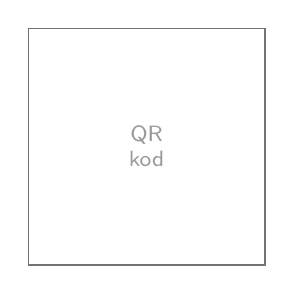
\begin{tikzpicture}
\draw[black!55,line width=0.6pt] (0,0) rectangle (30mm,30mm);
\node[black!40,font=\sffamily\fontsize{8}{9}\selectfont,align=center] at (15mm,15mm) {QR\\kod};
\end{tikzpicture}\\[1.5mm]
{\sffamily\bfseries\fontsize{9}{11}\selectfont\color{ink} #1}\\[1.5mm]
{\sffamily\fontsize{8.5}{11}\selectfont\color{black!45} @\makebox[20mm]{\dotfill}}%
}

\newcommand{\frontheader}[1]{%
\begin{textblock*}{194mm}(16mm,16mm)
\begin{tikzpicture}
\node[font=\sffamily\bfseries\fontsize{15}{16}\selectfont,text=ink,anchor=west] at (0,0) {#1};
\end{tikzpicture}
\end{textblock*}
\begin{textblock*}{194mm}(16mm,22.5mm)

\begin{tikzpicture}
\fill[accent] (0,0) rectangle (194mm,0.5mm);
\end{tikzpicture}
\end{textblock*}
}

\begin{document}

% ================= PAGE i: TITLE PAGE =================
\pagefooter{3}
\mbox{}%

\begin{textblock*}{160mm}(20mm,40mm)
{\sffamily\bfseries\fontsize{10}{12}\selectfont\color{ink} AVAZBEKOV SALOHIDDIN AZAMJON O'G'LI}
\end{textblock*}

\begin{textblock*}{3mm}(20mm,60mm)

\begin{tikzpicture}
\fill[accent] (0,0) rectangle (3mm,-110mm);
\end{tikzpicture}
\end{textblock*}

\begin{textblock*}{165mm}(32mm,58mm)
{\sffamily\bfseries\fontsize{48}{48}\selectfont\color{ink} SAT\\[2mm]1200+}
\end{textblock*}

\begin{textblock*}{150mm}(32mm,145mm)
{\sffamily\bfseries\fontsize{14}{18}\selectfont\color{accent} 3-KITOB \textperiodcentered\ $\approx$800}
\end{textblock*}

\begin{textblock*}{150mm}(32mm,158mm)
{\sffamily\fontsize{11}{15}\selectfont\color{ink} Master SAT tricks for perfect score}
\end{textblock*}

\begin{textblock*}{150mm}(20mm,255mm)
{\sffamily\fontsize{9}{13}\selectfont\color{black!55} Qisqa muddat ichida SAT uchun kerakli matematika\\va ingliz tili bilimlari}
\end{textblock*}

\newpage

% ================= PAGE ii: COPYRIGHT / LEGAL =================
\frontheader{Mualliflik huquqi}
\pagefooter{4}
\mbox{}%

\begin{textblock*}{170mm}(20mm,34mm)
{\fontsize{10.5}{16}\selectfont\color{ink}

\textbf{\copyright\ 2026 Avazbekov Salohiddin Azamjon o'g'li. Barcha huquqlar himoyalangan.}

\vspace{4mm}
Ushbu kitobning biron qismini muallifning yozma ruxsatisiz ko'paytirish, qayta chop etish yoki sotish qat'iyan taqiqlanadi. Kitobni elektron, fotonusxa, skanerlash yoki boshqa har qanday usulda nusxalash mualliflik huquqini buzish hisoblanadi va qonun bo'yicha javobgarlikka olib keladi.

\vspace{4mm}
Birinchi nashr --- 2026, Chartak, Namangan viloyati, O'zbekiston.

\vspace{2mm}
Chop etildi: Chartak ZiyoFoto Studio.

\vspace{6mm}
{\fontsize{9}{13}\selectfont\itshape SAT\textregistered\ is a registered trademark of the College Board, which was not involved in the production of, and does not endorse, this product.}

\vspace{8mm}
\begin{tabular}{@{}p{14mm}p{140mm}@{}}
Muallif: & Avazbekov Salohiddin Azamjon o'g'li \\[2mm]
Telegram: & @tripplezet \\[2mm]
Email: & avazbekovsalohiddin19@gmail.com \\[2mm]
Tel: & +998 94 206 00 19 \\
\end{tabular}
}
\end{textblock*}

\newpage

% ================= PAGE iii: ABOUT THE BOOK =================
\frontheader{Kitob haqida}
\pagefooter{5}
\mbox{}%

\begin{textblock*}{170mm}(20mm,34mm)
{\fontsize{11}{16}\selectfont\color{ink}

\textbf{SAT 1200+} --- Digital SAT imtihonining matematika bo'limiga tayyorlanish uchun yozilgan uch kitoblik seriya. \textbf{3-kitob} --- seriyaning cho'qqisi: eng qiyin savollarni yechish, vaqtni tejaydigan usullar va to'liq hajmli mock testlar orqali \textbf{≈800} ballga tayyorlanish.

\vspace{4mm}
Bu kitobda yangi mavzu emas, balki \emph{tanish mavzularning qiyin ko'rinishi} o'rgatiladi: qiyin SAT savollari odatda siz biladigan 2--3 qoidani zanjirga ulaydi yoki oddiy masalani g'ayrioddiy shaklda yashiradi. Barcha masalalar original, javoblari esa tekshirilgan; ular College Board'ning rasmiy savollar bazasi \emph{usullari} tahlili asosida yozilgan.

\vspace{4mm}
\textbf{Har bir darsning tuzilishi:}

\vspace{2mm}
\begin{tabular}{@{}p{10mm}p{150mm}@{}}
1. & \textbf{Qoida/Formula sahifasi (Rules sheet)} --- eng muhim qoidalar va usullar, qisqa misollar bilan; oxirida 10--15 ta yangi so'z (New words). QR kod orqali video darsni ko'ring. \\[3mm]
2. & \textbf{Mashqlar (Problems)} --- 5 ta to'plam: bosqichma-bosqich qiyinlashib, "Summit" to'plamida eng qiyin masalalar. \\[3mm]
3. & \textbf{Qaydlar uchun} --- har bir darsdan keyin o'zingiz yozib borishingiz uchun bo'sh sahifa. \\[3mm]
4. & \textbf{Javoblar (Answer key)} --- har bir masala uchun qisqa yechim va qo'llanilgan usul nomi. \\
\end{tabular}

\vspace{4mm}
Kitob oxirida \textbf{10 ta to'liq mock test} (har biri: 1-modul va qiyinroq 2-modul, 22 savoldan, 35 daqiqadan) berilgan. Mock testlarning javoblari testdan keyin emas, kitobning eng oxirida, \textbf{Answer sheets} bo'limida beriladi.

}
\end{textblock*}

\begin{textblock*}{170mm}(20mm,218mm)
{\sffamily\bfseries\fontsize{11}{14}\selectfont\color{ink} Bizni kuzating}
\end{textblock*}

\begin{textblock*}{170mm}(20mm,225mm)

\begin{tikzpicture}
\fill[accent] (0,0) rectangle (170mm,0.4mm);
\end{tikzpicture}
\end{textblock*}

\begin{textblock*}{170mm}(20mm,233mm)
\centering
\begin{minipage}[t]{30mm}\centering\qrbox{Telegram}\end{minipage}%
\hspace{20mm}%
\begin{minipage}[t]{30mm}\centering\qrbox{YouTube}\end{minipage}%
\hspace{20mm}%
\begin{minipage}[t]{30mm}\centering\qrbox{Instagram}\end{minipage}
\end{textblock*}

\end{document}
